\chapter{Results}
\label{chap:results}

\section{General Information}
\label{sec:general_info}
In total there were 120 participants in the study who made a submission according to Prolific. 12 were removed due to technical issues with the submissions, either their submission were not received due to technical issues or they actually did not fully complete the experiment. Another 3 were removed due to having missing data in some of the trials and another 4 were removed due to having accuracy on unambiguous trials below 75\% according to our preregistration. This left us with 101 participants for the analysis. 

It is worth noting that due to the nature of the experiment, the calibration was difficult to pass, making the experiment difficult to complete. 120 participants completed the experiment, however, the were around 150 submission attempts that were not completed. This mainly happened because of the calibration difficulties according to some of the participants feedback. This information gives us an idea about the completion rate of the experiment, which amounted at around 40\%. However, this allowed us to collect a large amount of good quality data, which is the most important aspect of the experiment.

Due to the complexity of the mixed effects models, convergence issues arised. Therefore, the random effects were removed one by one from the models based on the least variance among the random effects. The process was repeated until the models converged. In the case of predicting accuracy, the random effects were removed from the model entirely. 

\section{Pairwise Correlations}
\label{sec:pairwise_corr}

The pairwise correlations for the Simple and Complex conditions can be seen in \autoref{tab:correlation_table_simple} and \autoref{tab:correlation_table_complex} correspondingly. The correlations between the eye tracking features were excluded due to the way they were defined. Almost all of them have negative correlation because the features are proportional and increase in one of them means a decrease in some of the others. However, there was one exception to this general trend, it is a positive correlation between the \texttt{PropTimeOnDist} and \texttt{PropTimeOnNonAOI}, this indicates that 

\begin{table}[h!]
\centering
\begin{tabular}{|l|c|c|c|c|}
\hline
\textbf{Feature} & \textbf{Mean (SD)} & \textbf{Accuracy} & \textbf{Mean Answer Time} \\ \hline
PropTimeOnSentMsg & 0.29 (0.09) & -0.33 *** & -0.57 *** \\ \hline
PropTimeOnAvailableMsgs & 0.11 (0.07) & 0.35 *** & 0.38 *** \\ \hline
PropTimeOnTrgt & 0.24 (0.06) & 0.35 *** & 0.18 \\ \hline
PropTimeOnDist & 0.16 (0.06) & -0.03 & 0.29 ** \\ \hline
PropTimeOnComp & 0.18 (0.06) & -0.24 * & -0.07 \\ \hline
PropTimeOnNonAOI & 0.02 (0.01) & -0.02 & 0.04 \\ \hline
MeanAnswerTime (ms) & 5188 (2586) & 0.08 & --- \\ \hline
Accuracy & 0.8 (0.25) & --- & --- \\ \hline
\end{tabular}
\caption{Simple condition. Correlation table showing the relationships between features, accuracy, and mean answer time. Significance levels: * $p < 0.05$, ** $p < 0.01$, *** $p < 0.001$.}
\label{tab:correlation_table_simple}
\end{table}

\begin{table}[h!]
\centering
\begin{tabular}{|l|c|c|c|c|}
\hline
\textbf{Feature} & \textbf{Mean (SD)} & \textbf{Accuracy} & \textbf{Mean Answer Time} \\ \hline
PropTimeOnSentMsg & 0.26 (0.09) & -0.35 *** & -0.61 *** \\ \hline
PropTimeOnAvailableMsgs & 0.13 (0.07) & 0.22 * & 0.51 *** \\ \hline
PropTimeOnTrgt & 0.23 (0.07) & 0.56 *** & 0.02 \\ \hline
PropTimeOnDist & 0.15 (0.06) & -0.08 & 0.19 \\ \hline
PropTimeOnComp & 0.21 (0.06) & -0.26 ** & 0.11 \\ \hline
PropTimeOnNonAOI & 0.02 (0.02) & -0.01 & 0.01 \\ \hline
MeanAnswerTime (ms) & 6565 (4022) & 0.18 & --- \\ \hline
Accuracy & 0.7 (0.21) & --- & --- \\ \hline
\end{tabular}
\caption{Complex condition. Correlation table showing the relationships between features, accuracy, and mean answer time. Significance levels: * $p < 0.05$, ** $p < 0.01$, *** $p < 0.001$.}
\label{tab:correlation_table_complex}
\end{table}

\section{Predicting Accuracy}
\label{sec:accuracy_model}

The final formula for the model predicting accuracy was:
\begin{verbatim}
    Correct ~ Condition + TrgtPos + Trial + PropTimeOnTrgt +
    PropTimeOnComp + PropTimeOnDist + PropTimeOnSentMsg + 
    PropTimeOnAvailableMsgs + MsgType + AnswerTime + 
    Condition:PropTimeOnTrgt + Condition:PropTimeOnComp +
    Condition:PropTimeOnDist + Condition:PropTimeOnSentMsg +
    Condition:PropTimeOnAvailableMsgs + Condition:AnswerTime
\end{verbatim}
The model had the following encodings for the categorical variables \autoref{tab:msgtype_encoding}, \autoref{tab:trgtpos_encoding} and \autoref{tab:condition_encoding}. The target position can be interpreted as comparing left to the center and right to the center for features `TrgtPos1` and `TrgtPos2` respectively. The condition can be interpreted as comparing the simple condition to the complex condition and the unambiguous condition to the simple and complex conditions together. The model was trained using the \texttt{lme4} package in R. The model was trained using the \texttt{glm} function with the following parameters: \texttt{family = binomial(link = "logit")}. The resulting coefficients can be seen at \autoref{tab:model_coefficients_acc}. 

\begin{table}[h!]
    \centering
    \begin{tabular}{|c|c|}
    \hline
    Message Type & \textbf{MsgType} \\ \hline
    Shape        & -1       \\ \hline
    Color        & 1        \\ \hline
    \end{tabular}
    \caption{Encoding of the message type categorical variable.}
    \label{tab:msgtype_encoding}
    \end{table}
    \hfill
    \begin{table}[h!]
    \centering
    \begin{tabular}{|c|c|c|c|}
    \hline
    Target Position & TrgtPos1 & TrgtPos2\\ \hline
    0               & 1    & 0    \\ \hline
    1               & 0    & 0    \\ \hline
    2               & 0    & 1    \\ \hline
    \end{tabular}
    \caption{Encoding of the target position categorical variable.}
    \label{tab:trgtpos_encoding}
    \end{table}
    \begin{table}[h!]
    \centering
    \begin{tabular}{|c|c|c|}
    \hline
    Condition     & Condition1 & Condition2 \\ \hline
    Complex       & -1   & -1   \\ \hline
    Simple        & 1    & -1   \\ \hline
    Unambiguous   & 0    & 2    \\ \hline
    \end{tabular}
    \caption{Encoding of the condition categorical variable.}
    \label{tab:condition_encoding}
\end{table}


Looking at some general findings from \autoref{tab:model_coefficients_acc}, starting from the Intercept, it is positive and significant, indicating that having no information about any other features, the trial is more likely to be solved correctly. This is unsurprising as the average accuracy across all trials amounted at 82.5\%. 

One can see from \texttt{Condition1} that the Complex trials are predicted to have significantly lower accuracy comparing to the Simple ones. However, the effect is not fully captured by this coefficient due to the inclusion of the interaction terms. \texttt{Condition2} indicates that unambiguous trials have a higher probability of being solved correctly comparing to simple and complex ones, the effect is also significant. So far, the findings fully align with how the trials were designed. 

The target position is more of a not easy to interpret effects. The findings suggest that the when the target is on the left or right side, the probability of correctly answering increases, the effect is significant. This might be somehow related to the fact that the objects are split far apart from each other.

\begin{table}[h!]
\centering
\begin{tabular}{|l|c|c|c|c|}
\hline
\textbf{Coefficient} & \textbf{Estimate} & \textbf{Std. Error} & \textbf{z value} & \textbf{Pr(>|z|)} \\ \hline
(Intercept)                          & 1.23265 & 0.18460 & 6.677 & 2.43e-11 *** \\ \hline
Condition1                           & 0.22087 & 0.05499 & 4.017 & 5.91e-05 *** \\ \hline
Condition2                           & 1.10938 & 0.14302 & 7.757 & 8.69e-15 *** \\ \hline
TrgtPos1                             & 1.92305 & 0.21183 & 9.078 & < 2e-16 *** \\ \hline
TrgtPos2                             & 1.69844 & 0.20450 & 8.305 & < 2e-16 *** \\ \hline
Trial                                & 0.22635 & 0.04825 & 4.691 & 2.72e-06 *** \\ \hline
PropTimeOnTrgt                      & -6.09992 & 6.15675 & -0.991 & 0.3218 \\ \hline
PropTimeOnComp                     & -12.92581 & 6.16769 & -2.096 & 0.0361 * \\ \hline
PropTimeOnDist                     & -11.95582 & 6.14733 & -1.945 & 0.0518 . \\ \hline
PropTimeOnSentMsg                   & -9.95567 & 6.06806 & -1.641 & 0.1009 \\ \hline
PropTimeOnAvailableMsgs             & -8.69726 & 6.27784 & -1.385 & 0.1659 \\ \hline
MsgType                            & -0.11506 & 0.04888 & -2.354 & 0.0186 * \\ \hline
AnswerTime                          & -0.12537 & 0.05186 & -2.418 & 0.0156 * \\ \hline
Condition1:PropTimeOnTrgt           & -1.93730 & 1.09696 & -1.766 & 0.0774 . \\ \hline
Condition2:PropTimeOnTrgt          & -12.13074 & 6.12982 & -1.979 & 0.0478 * \\ \hline
Condition1:PropTimeOnComp           & -1.30711 & 1.08177 & -1.208 & 0.2269 \\ \hline
Condition2:PropTimeOnComp          & -11.30869 & 6.12510 & -1.846 & 0.0649 . \\ \hline
Condition1:PropTimeOnDist           & -1.13168 & 1.08619 & -1.042 & 0.2975 \\ \hline
Condition2:PropTimeOnDist          & -12.16270 & 6.10435 & -1.992 & 0.0463 * \\ \hline
Condition1:PropTimeOnSentMsg        & -0.97657 & 1.09161 & -0.895 & 0.3710 \\ \hline
Condition2:PropTimeOnSentMsg       & -10.26290 & 6.03306 & -1.701 & 0.0889 . \\ \hline
Condition1:PropTimeOnAvMsgs   & 0.70963 & 1.13710 & 0.624 & 0.5326 \\ \hline
Condition2:PropTimeOnAvMsgs & -12.08512 & 6.24131 & -1.936 & 0.0528 . \\ \hline
Condition1:AnswerTime               & -0.11566 & 0.05769 & -2.005 & 0.0450 * \\ \hline
Condition2:AnswerTime               & -0.02166 & 0.03973 & -0.545 & 0.5856 \\ \hline
\end{tabular}
\caption{Summary of the trained model coefficients. Significance codes: 0 '***', 0.001 '**', 0.01 '*', 0.05 '.', 0.1 ' ', 1.}
\label{tab:model_coefficients_acc}
\end{table}

The coefficent for \texttt{Trial} suggests that people get better as they progress through the experiment. This is expected as the participants have feedback after they answer, which tells whether their answer is correct or not. This finding also aligns with some of the findings from the previous work \cite{Mayn_2023, Mayn_2025}. 

Moving to the eye tracking features, the \texttt{PropTimeOnComp} has a significant negative effect, indicating that the more participant looks at the competitor, the more likely they are to answer incorrectly. This effect probably comes from the last look that people do before selecting the object which tips the proportional feature. If a participant cannot derive the correct answer through the reasoning, they will most likely guess among the Target and the Competitor as they both share the sent message feature, making looking at the Competitor negatively correlated to the accuracy.

Furthermore, the \texttt{PropTimeOnDist} has a large negative effect, it is almost significant. The effect is most likely coming from the Unambiguous trials which we will discuss later more in details. 

The \texttt{MsgType} indicates that trials where the sent message is a shape are more likely to be solved correctly. The effect is significant, although relatively small.

Regarding the \texttt{AnswerTime}, the general term suggests that the longer one stays on the trial, the more likely they are to answer incorrectly. However, this term should be interpreted together with the interaction terms. We will discuss it later in more details.


\begin{table}[h!]
\centering
\begin{tabular}{|c|c|c|c|c|}
\hline
\textbf{Condition} & \textbf{PropTimeOnDist.trend} & \textbf{SE} & \textbf{asymp.LCL} & \textbf{asymp.UCL} \\ \hline
Complex            & 1.339                        & 1.46        & -1.53              & 4.204              \\ \hline
Simple             & -0.925                       & 1.63        & -4.11              & 2.265              \\ \hline
Unambiguous        & -36.281                      & 18.30       & -72.13             & -0.434             \\ \hline
\end{tabular}
\caption{Trends for proportional time on Distractor based on condition.}
\label{tab:proptimeondist_trends}
\end{table}

\begin{figure}
    \centering
    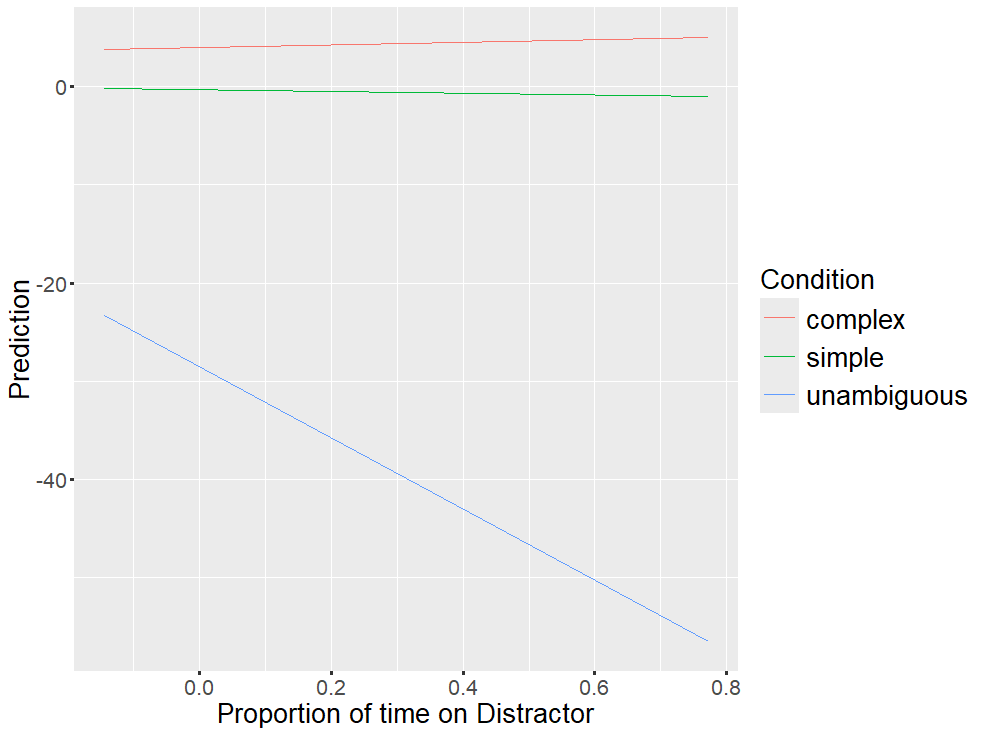
\includegraphics[width=0.8\textwidth]{images/proptimeondist_trends.png}
    \caption{Visualization of trends for proportional time on Distractor based on condition.}
    \label{fig:proptimeondist_trends}
\end{figure}

\begin{table}[h!]
\centering
\begin{tabular}{|c|c|c|c|c|c|}
\hline
\textbf{Contrast} & \textbf{Estimate} & \textbf{SE} & \textbf{z.ratio} & \textbf{p.value} \\ \hline
Complex - Simple & 2.26 & 2.17 & 1.042 & 0.5504 \\ \hline
Complex - Unambiguous & 37.62 & 18.30 & 2.051 & 0.1003 \\ \hline
Simple - Unambiguous & 35.36 & 18.30 & 1.927 & 0.1311 \\ \hline
\end{tabular}
\caption{Contrasts for proportional time on Distractor based on condition.}
\label{tab:proptimeondist_contrasts}
\end{table}

The first hypothesis we were interested in was that Proportional time on Distractor is positively associated with accuracy on Complex trials, described in \autoref{sec:h1}. Even though the coefficient for the interaction term `Condition1:PropTimeOnDist' is not significant, due to how interaction terms work, we can still interpret how model prediction changes based on the value of the interaction term. First of all, we can take a look at \autoref{tab:proptimeondist_trends} which shows the trends of the Proportional time on Distractor for each condition. As well as the plot \autoref{fig:proptimeondist_trends} which visualizes the trends of the Proportional time on Distractor for each condition. The \autoref{tab:proptimeondist_trends} indicates the trends we anticipated, however, the columns \texttt{asymp.LCL} and \texttt{asymp.LCL} indicate the asymptotic lower and upper confidence limits -- that is, the 95\% confidence interval around the slope estimate. In simple and complex cases the interval includes 0, making the slopes not significant. It is worth noting that the slope for the Unambiguous trials is very large and ends up as significant in the end. However, the main issue is that the amount of incorrectly solved Unambiguous trials is extremely low, as the average accuracy on Unambiguous trials amounted to 98\%. This fact makes the slope have very large standard error and subsequently the confidence interval is also very spread. Futhermore, we can look at \autoref{tab:proptimeondist_contrasts}. The table indicates the differences between the slopes and gives corresponding p values for them. The row corresponding to our hypothesis is the first one `Complex - Simple'. the findings indicate that the Complex trials will benefit more from the proportional time on Distractor than the Simple ones. However, again, the effect is not significant. In addition, the estimates for the contrasts that include Unambiguous trials are close to being significant, however, probably unreliable for the reasons we discussed earlier.

\begin{table}[h!]
\centering
\begin{tabular}{|c|c|c|c|c|}
\hline
\textbf{Condition} & \textbf{PropTimeOnAvMsgs.trend} & \textbf{SE} & \textbf{asymp.LCL} & \textbf{asymp.UCL} \\ \hline
Complex            & 2.68                                  & 1.51        & -0.281             & 5.64              \\ \hline
Simple             & 4.10                                  & 1.70        & 0.761              & 7.43              \\ \hline
Unambiguous        & -32.87                                & 18.70       & -69.502            & 3.77              \\ \hline
\end{tabular}
\caption{Trends for proportional time on available messages based on condition.}
\label{tab:proptimeonavmsgs_trends}
\end{table}

The second hypothesis goes as follows, proportional time on available messages is positively associated with accuracy on Simple trials, described in \autoref{sec:h2}. Similarly to how we interpreted the findings for the first hypothesis, we will look at the actual predictions of the model and not solely at the coefficients to capture the whole relation between the interaction terms and the regular ones. First of all, the trends table is presented at \autoref{tab:proptimeonavmsgs_trends}. From the table we can indeed see a positived effect of proportional time on available messages on Simple condition. Therefore, the findings support the second hypothesis. In addition, the confidence interval does not include 0, suggesting that the effect is significant. As for the Complex and unambiguous trials, neither of the effects are significant, however, the trend for the Complex trial is also positive, suggesting that the available messages are still important for the participants in the Complex trials. It is worth noting, that the Complex trials can be solved without knowing the available messages at all as was described in \autoref{sec:h2}. Hence, the avaialbe messages might not be as important in the Complex condition.


Taking into account the fact that \texttt{AnswerTime} and one of the interaction terms including it have significant effects, we will also interpret the trends for this feature.  The trends can be seen in \autoref{tab:answertime_trends}. From the table we can conclude that the answer time on the Simple condition has a significant negative effect. This means, that the longer one takes to solve the simple case, the more likely they are to answer incorrectly. The slopes for the other conditions are not significant.

\begin{table}[h!]
\centering
\begin{tabular}{|c|c|c|c|c|}
\hline
\textbf{Condition} & \textbf{AnswerTime.trend} & \textbf{SE} & \textbf{asymp.LCL} & \textbf{asymp.UCL} \\ \hline
Complex            & 0.012                     & 0.0678      & -0.121             & 0.1449             \\ \hline
Simple             & -0.219                    & 0.0938      & -0.403             & -0.0356            \\ \hline
Unambiguous        & -0.169                    & 0.1040      & -0.372             & 0.0351             \\ \hline
\end{tabular}
\caption{Trends for Answer Time based on condition.}
\label{tab:answertime_trends}
\end{table}

\section{}
